\documentclass[11pt]{scrartcl}
\usepackage{answers}
\Newassociation{sketch}{hintitem}{hints}
\renewcommand{\solutionextension}{out}

\usepackage[sexy]{evan}
\newcommand\EE{\mathbb E}
\newcommand\PP{\mathbb P}
\usepackage{graphicx}
\usepackage{wrapfig}
\begin{document}
\title{Image Depth Estimation Using Stereo Vision}
\author{Mrinall Umasudhan}
\date{April 25, 2022}
\maketitle
\Opensolutionfile{hints}

\begin{abstract}
	Candidate ID: \mailto{943289432}.
\end{abstract}

%TOC
\tableofcontents

% EV.pdf
% ploh handouts

\newpage

\section{Introduction}
One of the most explored problems in the field of computer vision is the process
of accurately estimating the real-world depth of a pixel within a two dimensional
image. The inference of three dimensional information is done by using multiple two
dimensional views of a scene, the process being deemed the name stereo vision. 

\subsection{Applications}
A common counter-argument to the practicality of stereo vision algorithms 
are the presence of other sensors that do not make use of visual data such 
as ultrasonic or time of flight distance sensors. While these sensors are not
not impacted by factors that would be detrimental to the accuracy of stereo 
vision algorithms such as the lack of adequate lighting,  
"stereo vision has the advantage that it achieves the 3-D acquisition without 
energy emission or moving parts" (https://research.csiro.au/qi/stereo-vision/). Moreover,
whereas traditional distance sensors focus on a singular point in space, stereo vision 
algorithms are only limited by the camera's field of view, making the depth analysis
large area far more simple and cost effective. Finally, stereo vision algorithms are able 
to easily work in conjunction with other 
computer vision techniques such as machine learning based object detection
models when compared to the previous depth estimation approaches as it already
tracks depth on the same image plane that a object detection model may be implemented on.
These factors allow for a far greater analysis of the 
various shapes and angles in an image leading to its usage in various fields. 
\\ 
\begin{wrapfigure}{R}{0.5\textwidth}
\centering
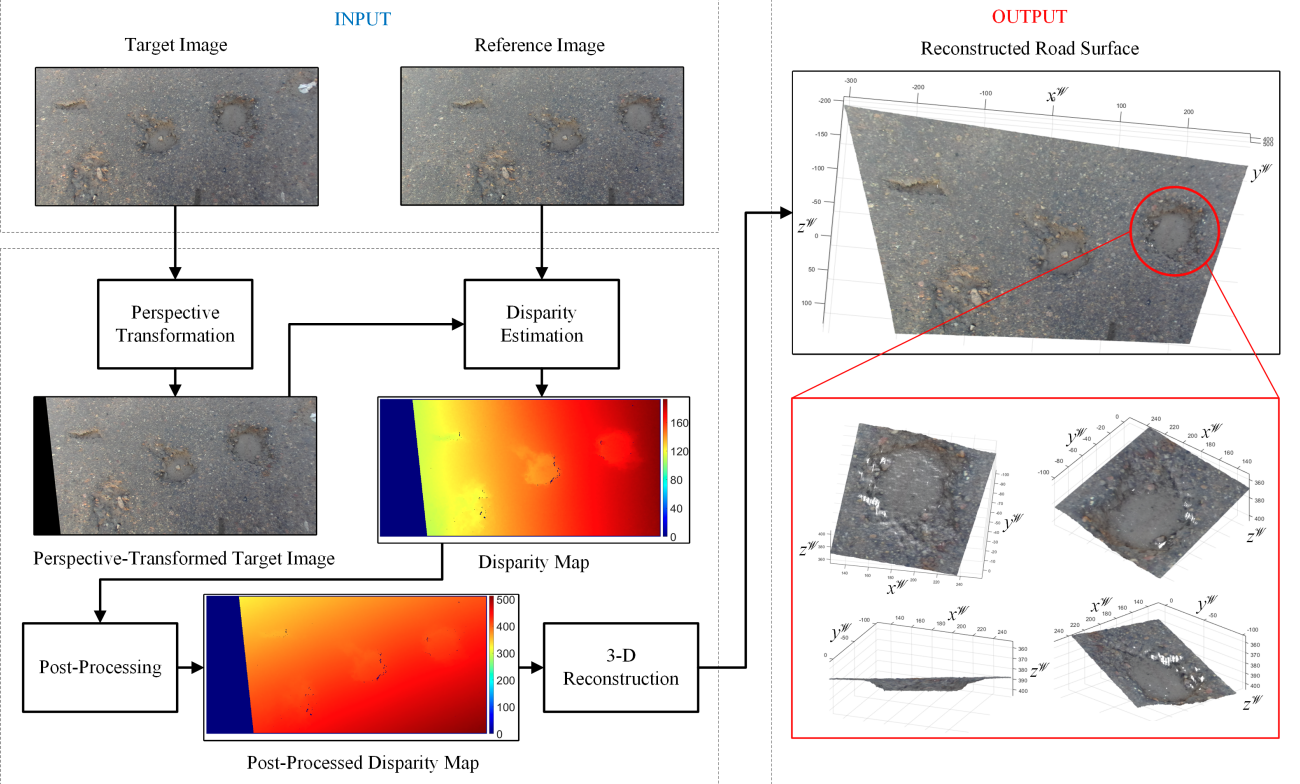
\includegraphics[width=0.5\textwidth]{img1.png}
\caption{\label{fig:frog1}Stereo Vision For Road Deformity Detection}
\end{wrapfigure}

A common application of stereo vision algorithms is in the quality
control process of industrial factories. Factories must analyze each
finished product for deformities in order to maintain a standard of quality in their 
products. However, many factories output a high volume of product every day meaning that
the human analysis of such product would be far too expensive and inefficient when
considering the large amounts of workers needed to manually inspect each products
as well as the time it takes for the inspection of a product. The installation of multiple
distance sensors in order to analyze each square inch of a product would also be far too expensive. 
However, because a factory is in a controlled environment with uniform lighting and the object is one
of known shape, the usage of a stereo vision algorithm would be ideal for the situation as stereo cameras 
are able to analyze objects with their large field of view and can easily detect deformities as the object 
being analyzed is of known geometry, meaning the algorithm can compare each depth point of the current object 
to the depth of a model product, reporting any deformities both accurately and efficiently.  and can easily detect deformities as the object 
being analyzed is of known geometry, meaning the algorithm can compare each depth point of the current object 
to the depth of a model product, reporting any deformities both accurately and efficiently. \\

A paper done by the University of Bristol explored deformity analysis preformed by stereo algorithms
further by acquiring three dimensional road data for autonomous cars further displaying the 
capabilities of stereo algorithms. The process which this algorithm follows can be seen in the 
figure above. 

\subsection{Overview and Purpose}

The essence of many successful stereo vision algorithms can be summarized in three key steps:
{\begin{enumerate}

    \item Triangulation: The process of assigning depth values to each pixel in the image 
        using multiple two dimensional views of a scene and the specific parameters from
        camera hardware, difference in location of the cameras used, and the disparity in the 
        pixels from each view of the scene.
    \item Calibration: The process of correcting image distortion caused by the 
        spherical geometry of the camera lens 
        and reifying the two dimensional views of the scene such that 
        the objects in study are on the same plane. 
    \item Pixel Correspondence: In order to apply the triangulation process the algorithm must be 
        able to match a pixel from one view of the scene to another view taken from a separate camera 
        also known as the disparity value of this pixel.  
\end{enumerate}}

\\

In modern research, the most studied step of the algorithm is the process of pixel Correspondence, 
better known as stereo matching. As of now there are many optimization techniques being applied 
to stereo matching algorithms in order to increase their efficiency and accuracy. Firstly, this paper explains 
the math and logic behind each portion of a successful stereo vision system while providing implementations.  finding value in optimization techniques 
when compared to more standard stereo matching approaches. In order to analyze and implement a sound stereo vision algorithm 
as well as a optimized matching algorithm scholarly sources were regarding stereo vision and optimization 
techniques for pixel correspondence. After implementing a standard matching algorithm as well as another using 
the optimization technique known as dynamic programming, I found that there was a significant increase
in both accuracy and efficiency in the depth estimates provided from the algorithm. 


\section{Triangulation}
Core of the algorithm

\subsection{Forward Projection Model}
\begin{remark}
    % paragraph paragraph name (end)
    Notes{\begin{enumerate}
        \item First to know how to map 2d to 3d, the traditional Forward Imaging model must be understood. 
        \item Go over the pinhole model, projection matrix (world to camera and camera to pixel) simplified to the projection formula
        \item We can use this simplified formula to derive the distance of the pixel in an image by using two cameras
        \item This new formula is ... , take note of the (xl-xr) which indicates the difference in pixel position from the left and right camera
            this is known as \textbf{disparity}
        \item However, in order to attain accurate disparity values from the two cameras, they must be calibrated 
    \end{enumerate}} % (fold)
    \label{par:Notes}
    
    % paragraph paragraph name (end)
\end{remark}

\subsection{Derivation of Backwards Projection Model}


\section{Camera Calibration}

\subsection{Intrinsic matrix}
\begin{remark}
    % paragraph paragraph name (end)
    Notes{\begin{enumerate}
        \item  External Parameters: Position and Orientation of the camera with respect to the world coordinate frame\dots
        \item Internal Parameters: How the camera maps world points into the image coordinate frame.
        \item For the case of this program becuase of camera model was constructed to match an ideal model, we only need to make use of two variables the focal length and the distnce between the two cameras d.
        \item Use this as a good guide for the process: https://medium.com/swlh/i-see-you-computer-vision-fundamentals-64cc662d0b05. 
            Essentianlly use an mage of known geometry and rearange the original projection eqations to find both the fx anf fy
        \item In many modern cameras, the lenses are contructed in such a manner that pixel quality is maximized, however the shape of these lense
            can lead to singificant distortion in the image taken when compared to the true real world position. 
        \item There consists of two types of distortion \textbf{radial and tangential} 
        \item In the paper you can describe the correction equation as well as what they algo:ref
            but in the actual Implementation you would have to use the built in function since a custom distorition function is way to complex
            , have a custom intrinsic and extrinsic matrix computation tool though. 
    \end{enumerate}} % (fold)
    \label{par:Notes}

\subsection{Extrinsic Parameters}

\subsection{Lens Distortion}

    \subsubsection{Radial Distortion}
    \subsubsection{Tangential Distortion}

    
    % paragraph paragraph name (end)
\end{remark}

\section{Stereo Rectification}

\subsection{Window Based SSD Disparity Estimation}
\subsection{Adaptible Window Optimizations}
\begin{remark}
    % paragraph paragraph name (end)
    Notes{\begin{enumerate}
        \item Now that the two cameras have been calibrated such that they are on a identical image plane wiht one another you can now find the disparity between pixels of the two images in order to find depth using the triangulation model. 
        \item One way this may be done is through a window based method, where we search for the object selected in one image the seocnd by creating a window and linearly searching for identical pixels on the second image. This method may be done efficiently due to camera calibration as the pixel range is on the same scan line. 
        \item We can explore other methods of stereo rectification if we have time as the computation is pretty simple. You would have the use
            a minimmum squared difference algorithm on the average intensity of the window. 
    \end{enumerate}} % (fold)
    \label{par:Notes}

    
    % paragraph paragraph name (end)
\end{remark}

\subsection{Dynamic Programming Based Disparity Estimation}

\section{Implementation}

\subsection{Hardware}
\subsection{Program}

\section{Testing}

\section{Conclusion}

\section{Works Cited}

\section{Appendix}

\end{document}
